\documentclass[10pt,a4paper]{report}
\usepackage[utf8]{inputenc}
\usepackage[left=2cm,
			right=2cm,
			top=3cm,
bottom=3cm]{geometry}
\usepackage{amsmath}
\usepackage{amsfonts}
\usepackage{amssymb}
\usepackage{graphicx}
\usepackage{csvsimple}
\usepackage{placeins}
\usepackage{array,booktabs}
\usepackage[colorlinks=true,urlcolor=cyan]{hyperref}
\usepackage{listings} %code highlighting
\author{Cyril Matthey-Doret}
\begin{document}
\title{\textbf{Master Project}\\ Lab book}
\maketitle
\chapter{Introduction}

The goal of this project is to identify the locus or loci responsible for sex determination in the parasitoid wasp \textit{Lysiphlebus fabarum}. The species is known to have CSD, which means there are one or more loci that need to be heterozygous in order to triggger female development. I will use the offspring of asexual (thelytokous) females to identify these loci. The offspring consists of haploid males, diploid males and diploid females. Using DNA sequencing data, I will exclude haploid males as they do not provide information on homozygosity/heterozygosity and compare only diploid males versus females to identify the CSD locus/loci.
\textit{Lysiphlebus fabarum} wasp specimens (generation F4) issued from thelytokous mothers (generation F3) are used. These individuals come from crossing experiments in a strongly inbred line. Here, we use restriction site associated DNA sequencing(RAD-seq) with a custom pipeline to locate the locus/loci. Samples were single-end sequenced using a ddRAD protocole and digested with ecoRI and mseI. There are 2 separate libraries with two different illumina adaptors (detailed in next section). Statistics for the raw RAD-seq data of both libraries of F4 individuals are shown in table \ref{table:raw_QC}. I also reused sequencing data for the mothers (F3) from Casper, however I don't have the raw reads statistics as they were already processed.

\begin{table}[h]
\begin{center}
\begin{tabular}{l| c c}
 \multicolumn{1}{r}{Data summary:} \\
 \hline
library & lib7 & lib7b \\
raw reads & 163,506,603 & 133,574,055 \\
containing adaptors & 23.25\% & 45.84\% \\
fragment size & 302bp & 302bp \\
mean quality score & 34.88 & 35.05 \\
$>=$ Q30 bases & 92.62\% & 92.13\% \\

\end{tabular}
\caption{Summary statistics of raw reads from the 2 libraries of F4 individuals RAD-seq data.}
\label{table:raw_QC}
\end{center}
\end{table}

This lab book will document my progression for mapping the CSD locus, which can be broken down into 4 main steps: preprocessing of sequencing data, STACKs analysis for RAD-seq data, association mapping and orthology search. These steps are likely to change and throughout the project and it is likely that more will be added. The general process is described visually in figure \ref{pipeline}.
\begin{figure}
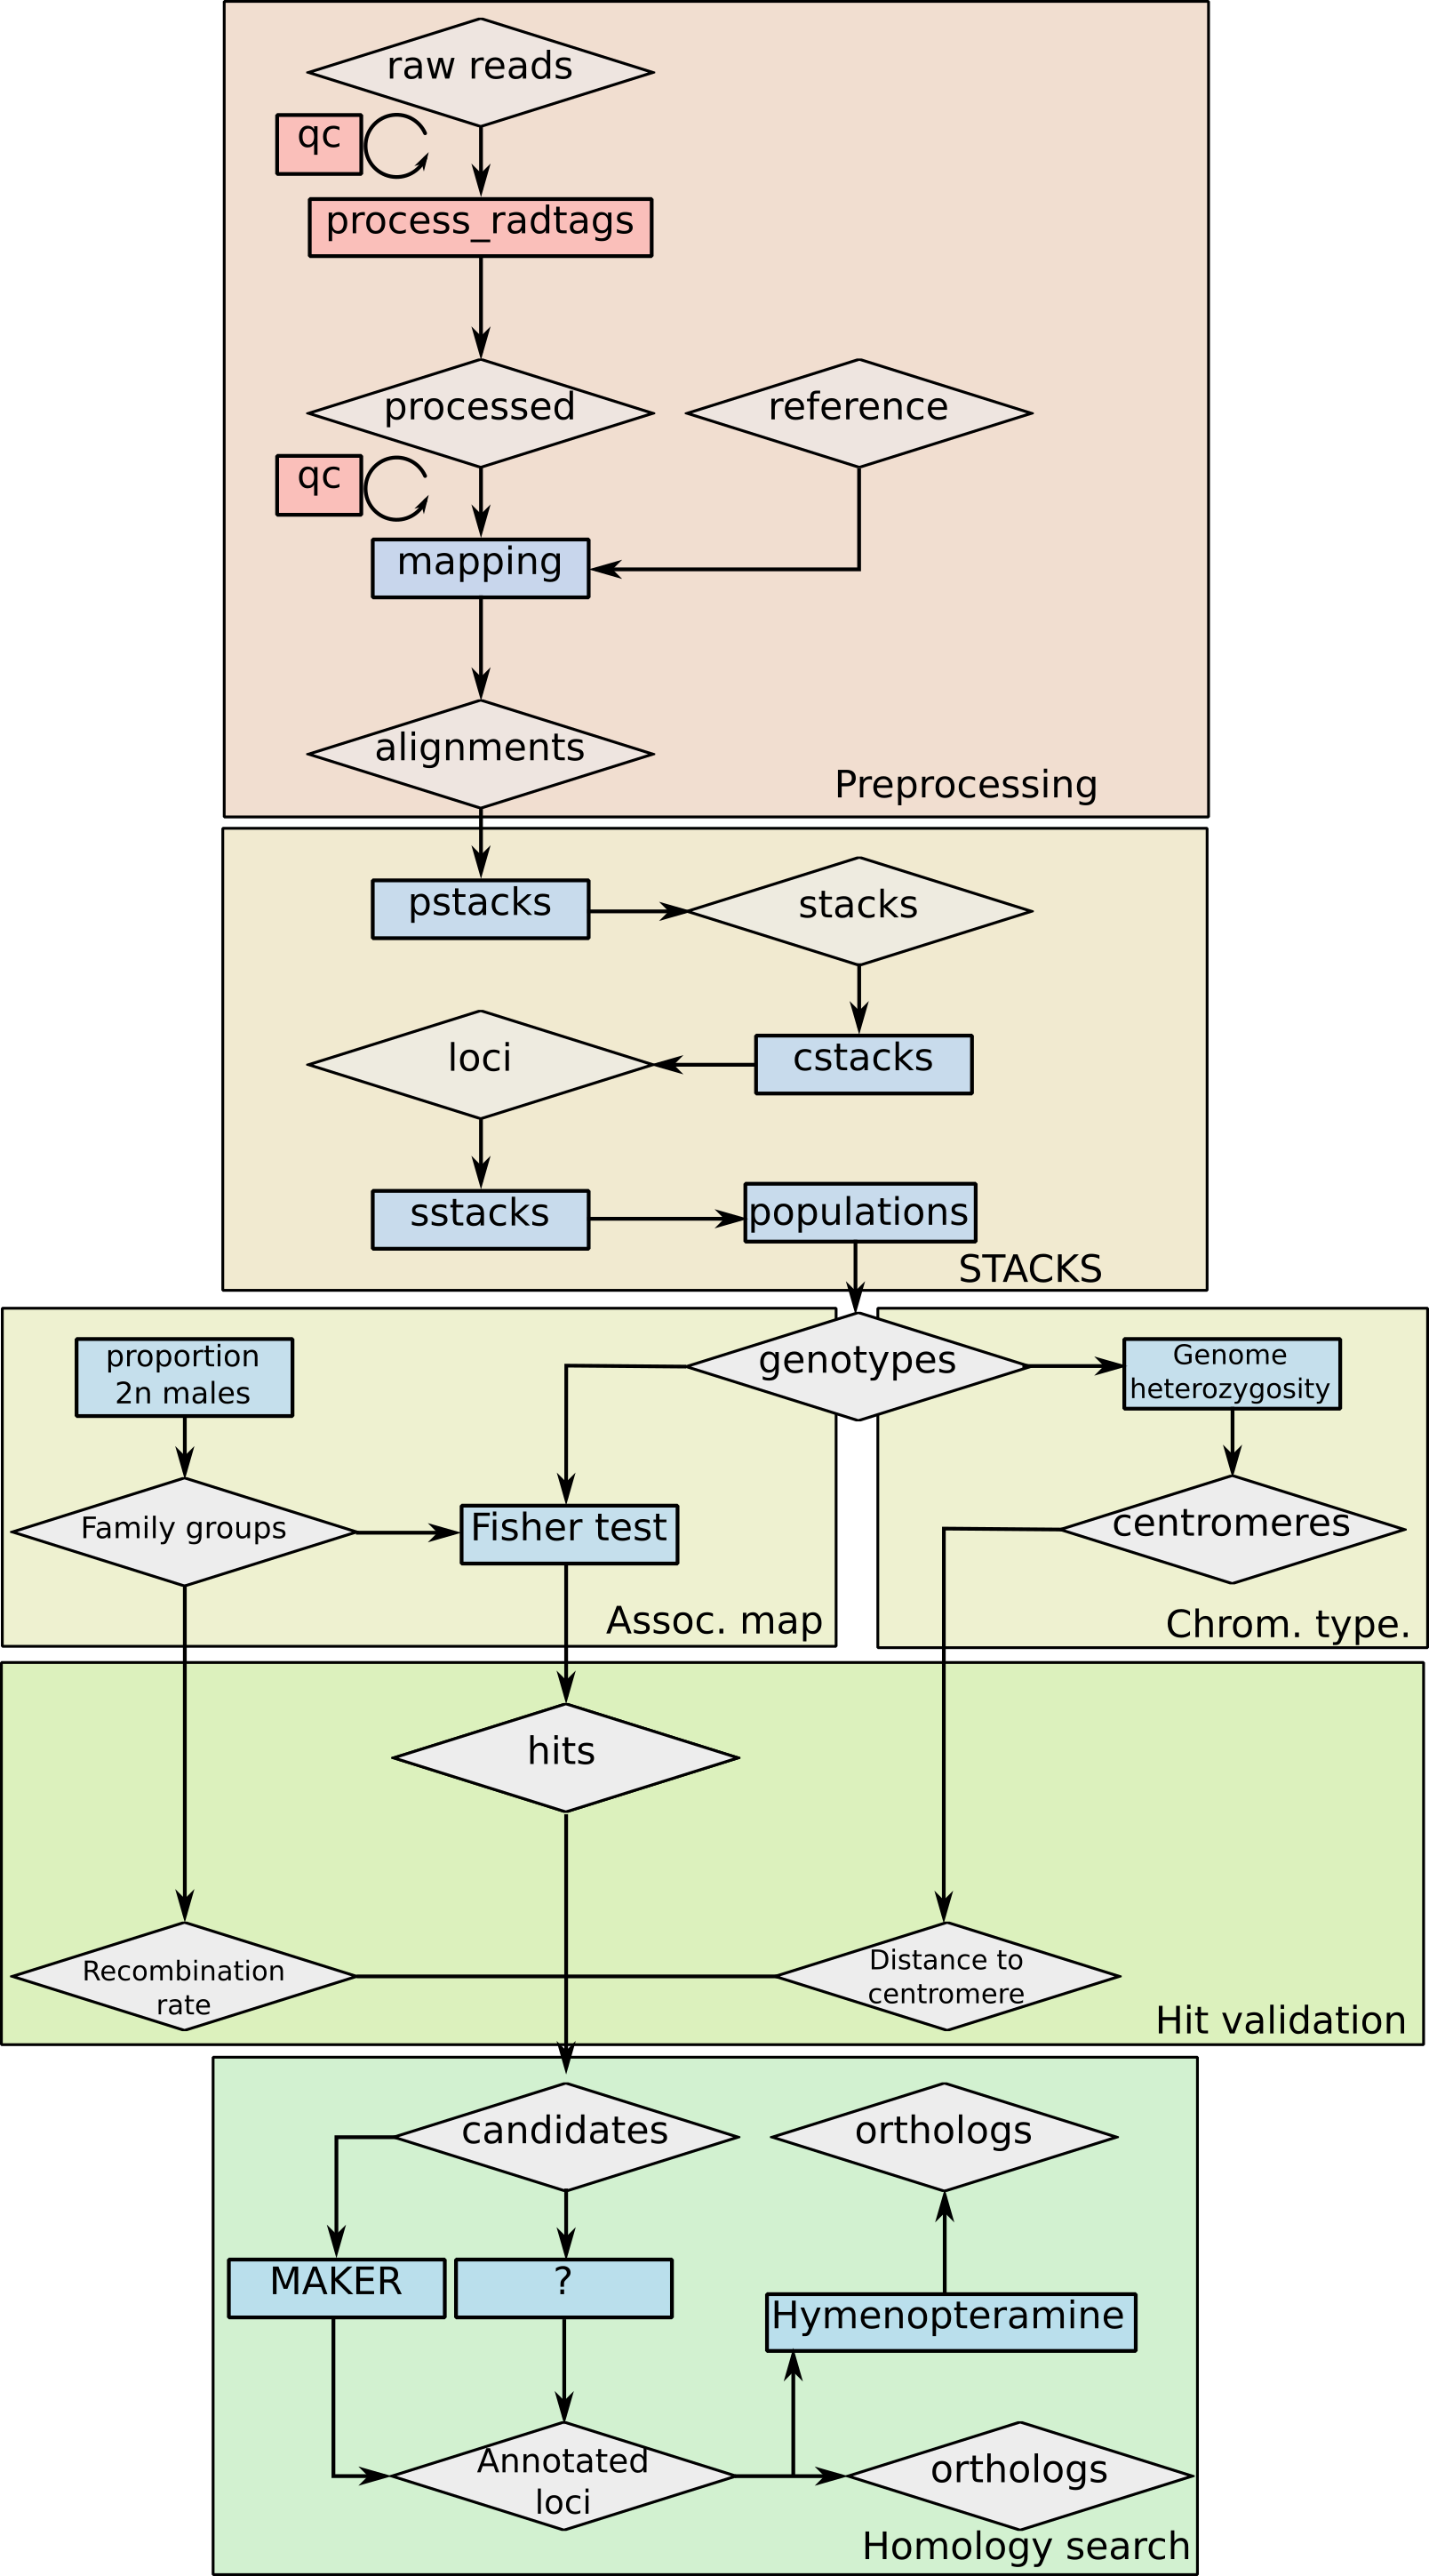
\includegraphics[scale=0.5]{flowchart}
\caption{\textbf{Pipeline described in the current lab book}. Diamonds represent data, rectangles represent operations/programs. Operations/programs in blue are included in the makefile, thos in red are not.}
\label{pipeline}
\end{figure}

 \chapter{Processing reads}
 RAD-seq data was split into 2 separate libraries: 7 and 7b. Together, the libraries contain 173 F4 individuals from 11 different F3 mothers. There were 96 samples in library 7 (one of which was contaminated) and 77 in library 7b. In total we have 172 valid samples across 11 families. Additionally, I inherited from 28 individuals from another library (lib6) which are offspring from families A and B.
 \section{Quality control}
 fastqc was used for quality control, separately on each file, and on all files together in the library.
 \section{Demultiplexing}
 The process-radtags program from stacks was used for demultiplexing and removal of Illumina adaptors. The operation was performed separately for libraries 7 and 7b:

\begin{lstlisting}
$ process_radtags -p raw/ -o processed/ -b \
/barcodes -e ecoRI --filter_illumina -E phred33 \
 -r -c -q --adapter_1 adapter --adapter_mm 2
\end{lstlisting}


\begin{center}
\begin{tabular}{c c}
lib7 & Truseq adapter, index 6 \footnotemark\\ 
lib7b & TruSeq adapter, index 12 \footnotemark\\
\end{tabular}
\end{center}
\footnotetext[1]{GATCGGAAGAGCACACGTCTGAACTCCAGTCACGCCAATATCTCGTATGCCGTCTTCTGCTTG}
\footnotetext[2]{GATCGGAAGAGCACACGTCTGAACTCCAGTCACCTTGTAATCTCGTATGCCGTCTTCTGCTTG}
\section{Trimming adaptors}
This step is performed by process radtags at the same time as demultiplexing. I tried different values for adapter mismatches, between 0 and 3 (i.e. reads containing sequences distant from the adapter by n mismatches are removed). This did not cause any major difference and therefore I will perform all downnstream analyses with an allowance of 2 mismatches in the adapter.

Note: Demultiplexing did not yield any read for CF4F10. 

\chapter{STACKS pipeline}

The pipeline described in this chapter will map the processed reads to the reference genome and build a catalogue of loci. It will eventually implement additional features such as calculating population statistics. At each step of the pipeline, I will try different combinations of parameters and choose the one yielding the best results. 

\section{Mapping}
Since the reference genome of \textit{Lysiphlebus fabarum} was recently released, I will first map the sequencing reads to the reference, using BWA, but I may also want to use bowtie to compare the results, eventually. At the moment, a draft reference genome is available, table \ref{assembly_stats} displays some summary statistics of it.
\begin{table}
\vspace{10px}
\csvautobooktabular[respect underscore=true]{stacks_pipeline/ref_genome_stats.csv}
\caption{Assembly statistics for the current reference genome of \textit{Lysiphlebus fabarum}}
\label{assembly_stats}
\vspace{10px}
\end{table}

\subsection{BWA}

BWA provides 3 different algorithms: MEM, backtrack (aln) and SW. MEM is normally the better for Illumina reads longer than 70bp, therefore I will be using this one here. Backtrack is preferred for short reads and SW with frequent gaps.
There are also 2 algorithms for building the index: 'is' and 'bwtsw'. 'is' is used with reference <2GB, 'bwtsw' with larger references.

General commands: 
\begin{lstlisting}
$ bwa index -p <out_index_name> -a <algorithm>
$ bwa mem <index> <sample.fq> > <out.sai>
> $sample-$prefix.sam
\end{lstlisting}

When using bwa-aln, there the command running the alignment (after indexing) is:
\begin{lstlisting}
$ bwa aln -n <mismatches> $index <sample.fq> > <sample.sai>
$ bwa samse -n <max_dupl> $index $sample.sai $data_dir/$sample.fq.gz
\end{lstlisting}
The first command (bwa index) constructs an index from the reference genome, whereas the second one (bwa mem/aln) actually runs the aligner. The third command (bwa samse) allows to transform the .sai into .sam files.

Here is the list of different mapping parameters I may try with bwa-mem:
\begin{itemize}
\item -k : minimum seed length (will miss matches shorter than value)[19]
\item -w : band width (gaps longer than value will not be found)[100]
\item -d : maximum distance between query and reference positions before stopping seed extension. [100]
\item -r : triggers reseeding for a MEM longer than min\_seed\_len$*$float. Larger values yield fewer seeds $->$ faster alignment but lower accuracy [1.5].
\end{itemize}

In the case we use the backtrack (aln) algorithm instead of MEM, the only parameter worth tuning is -n, the number of mismatches allowed. 


Note: I did not include parameters that are not relevant to sensitivity (e.g. threads) or parameters that involve scoring (changing these naively would probably have a negative impact). Full list of parameters is on the \href{http://bio-bwa.sourceforge.net/bwa.shtml}{official bwa website}

Note2: About multiple hits and BWA-mem: 

(https://github.com/lh3/bwa)

2. Why does a read appear multiple times in the output SAM?

BWA-SW and BWA-MEM perform local alignments. If there is a translocation, a gene fusion or a long deletion, a read bridging the break point may have two hits, occupying two lines in the SAM output. With the default setting of BWA-MEM, one and only one line is primary and is soft clipped; other lines are tagged with 0x800 SAM flag (supplementary alignment) and are hard clipped.


\subsection{Bowtie2}
General commands: 
\begin{lstlisting}
$ bowtie2-build reference_genome.fa L_fabarum
$ bowtie2 -x <ref_index> -U <unpaired_reads_files> -S <out_SAM_file>
\end{lstlisting}
The first command (bowtie2-build) constructs a set of index (extension: .bt2) from the reference genome, whereas the second one actually runs the aligner.

Here is the list of different mapping parameters I may try:
\begin{itemize}
\item --trim5 <n> : trim n bases from the 5' end (left) of each read before alignment
\item --trim3 <n> : trim n bases from the 3' end (right) of each read before alignment
\item -D : maximum number of seed extension that can fail in a row before stopping (increasing makes bt2 slower)
\item -R : maximum number of re-seeding when attempting to align read with repetitive seeds (increasing makes bt2 slower)
\item -N : number of mismatches permitted per seed (increasing reduces false negative, but makes bt2 slower)
\item -L : length of seeds (decreasing makes bt2 slower but more sensitive)
\item -i : interval between seeds (increasing makes bt2 slower but more sensitive)
\end{itemize}

Recommandations from the bowtie2 website to make alignment more sensitive: 
a) make seeds closer (reduce i)
b) make seeds shorted (reduce L)
c) allow more mismatches per seed

End-to-end versus local alignment (--local): end to end takes all bases in the reads into account, while local allows to trim reads to exclude the ends from the alignment.
Seeds are substring of the reads which bowtie2 tries to align to narrow down the valid regions for aligning a read. There is a list of preset values for these parameters on the \href{http://bowtie-bio.sourceforge.net/bowtie2/manual.shtml#preset-options-in---end-to-end-mode}{official bowtie2 website}. Preset parameters differ between local and end-to-end modes.
There are other parameters, such as score weights for gaps mismatches and allowance for 'N' ambiguous characters but changing these naively could probably have negative effect on the alignments.
Procedure: try out different preset values and select the one yielding the best results. Then, eventually tweak the parameters slightly from the preset values. These simulations can be run on a subset of individuals to speed up the process.

note to self: at the end of a run, bowtie2 prints a summary to stderr such as:

20000 reads; of these:

  20000 (100.00\%) were unpaired; of these:
  
    1247 (6.24\%) aligned 0 times
    
    18739 (93.69\%) aligned exactly 1 time
    
    14 (0.07\%) aligned $>$1 times
    
93.77\% overall alignment rate
\vspace{10px}\\
If I use Bowtie2, I will redirect the stderr and parse it into a csv file and generate plot to visually estimate the best parameter values.

\subsection{Mapping results}

I used the aln algorith of bwa, since the mem algorithm did not report multiple alignments and has very few documentation available. I tried different mismatches values with aln (Figure \ref{map_results}), ranging from 0 to 8, and I chose to use 4 since the increase in single was quite low above this value. When the mismatch parameter is set to 4, running bwa-aln on a subset of 12 samples yielded 57\% of single hit reads, 26\% of multiple hits and 17\% of unmapped reads.

\begin{figure}[h]
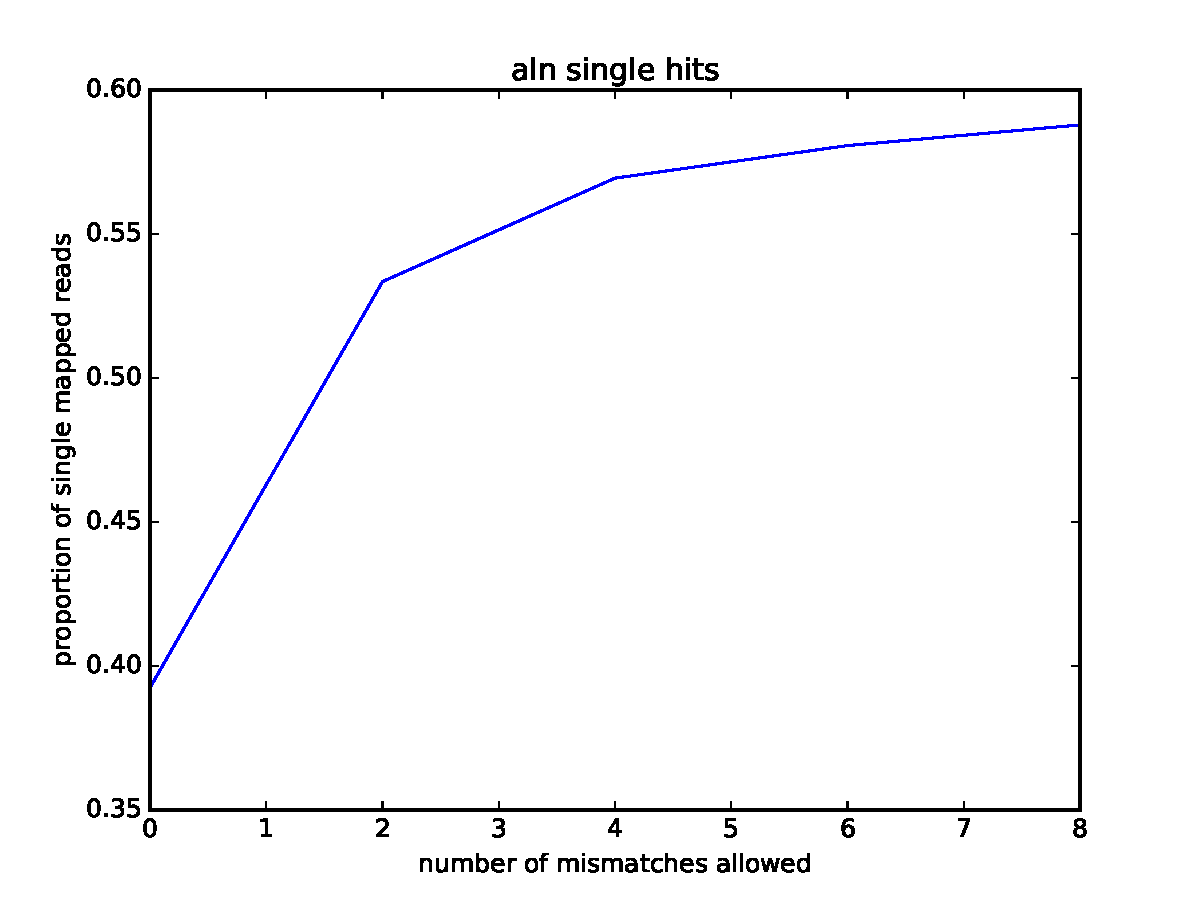
\includegraphics[scale=0.5]{param_space/mapstats}
\caption{Results of the BWA mapping with different parameter values for the number of mismatches allowed during mapping. The plot shows the proportion of reads that are mapped uniquely to the reference genome.}
\label{map_results}
\end{figure}

\section{pstacks}

pstacks is a component of the STACKS suite that takes stacks of reads aligned to a reference genome as an input (typically in the SAM format) and idenify SNPs

general command: 
\begin{lstlisting}
$ pstacks -f <input_path> -i <sample_ID_int> -o <out_dir> \
 -m <min_depth> -p <num_threads> -t <file_type>
\end{lstlisting}

Parameters I may want to change are: 
\begin{itemize}
\item -m : minimum depth of coverage required to call a stack [3]
\item --max\_clippped : alignments with more than X soft-clipped bases are discarded [15\%]
\item --min\_mapq : minimum required quality [10]
\end{itemize}

Note: there are 3 models; SNP, bounded SNP and fixed. SNP is the default model, bounded SNPs allows to give prior expectations about the error rate, which can allow better estimations of heterozygosity and the fixed model identifies all fixed sites and masks all others.

\subsection{pstacks results}

Pstacks was run on aligned reads (BWA, 4 mismatches allowed). I tried different values for the minimum coverage required to call a stack (-m parameter), ranging from 1 to 6 (Figure \ref{pstacks_param}). Below is the value for minimum coverage, along with the mean number of loci and alleles that was produced per sample. This table was produced including all non-empty samples (198 individuals) and the variables are averaged (arithmetic mean) over all those samples.

\begin{table}
\begin{center}
\vspace{10px}
\csvautobooktabular[respect underscore=true]{param_space/pstats.csv}
\vspace{10px}
\caption{Summary statistics of stacks obtained with different parameter values for minimum coverage in pstacks.}
\label{pstacks_param}
\end{center}
\end{table}

I will use 4 reads minimum coverage as this is already high and using lower values does not improve the output in anyway.

Note: Locus are regions formed by one or more stacks. Alleles are different stacks at the same locus.

\section{cstacks}

cstacks is a component of the STACKS suite that builds a catalog of loci with different alleles from a set of processed samples.

general command: 
\begin{lstlisting}
$ cstacks -s <sample_prefix> -o <out_dir> -b <catalogue_ID>\
-p <num_threads> -n <num_mm> -M <pop_map>
\end{lstlisting}

Parameters I may want to change are: 
\begin{itemize}
\item -n : Number of mismatches allowed between sample loci when building catalogue [1]
\item -g : base catalog on alignment position instead of sequence identity
\end{itemize}

Note: There are also advanced options such as gapped assembly parameters and loci matching multiple catalogue entries, but these are probably not relevant here.
\subsection{cstacks results}

I changed the number of mismatches allowed between samples between 1 and 4. Table \ref{cstacks_param} shows the results with a subset of 11 samples $([A-L\&\&[\wedge B]]01)$ because B01 was empty (few, low quality reads). 

\begin{table}
\begin{center}
\vspace{10px}
\csvautobooktabular[respect underscore=true]{param_space/cstats.csv}
\vspace{10px}
\caption{Summary statistics of loci obtained with different parameter values in cstacks.}
\label{cstacks_param}
\end{center}
\end{table}

I tried running cstacks on all (non-empty) samples, and also modifying the script so that it will first compute the mean number of tags (reads) across all samples, and exclude those with less than 10\% of this value when building the catalogue. From the 202 original samples, 4 were empty and excluding low quality ones removed 13 additional ones.\\

Update: 21.07.2017\\
When including mothers, I reach a total of 212 individuals. I use the same filtering strategy to exclude samples with low amounts of reads (Figure \ref{tags_dist}). From the 212 original samples, I excluded 17 low quality samples, among which 4 were totally empty.

\begin{figure}[h]
	\begin{center}
		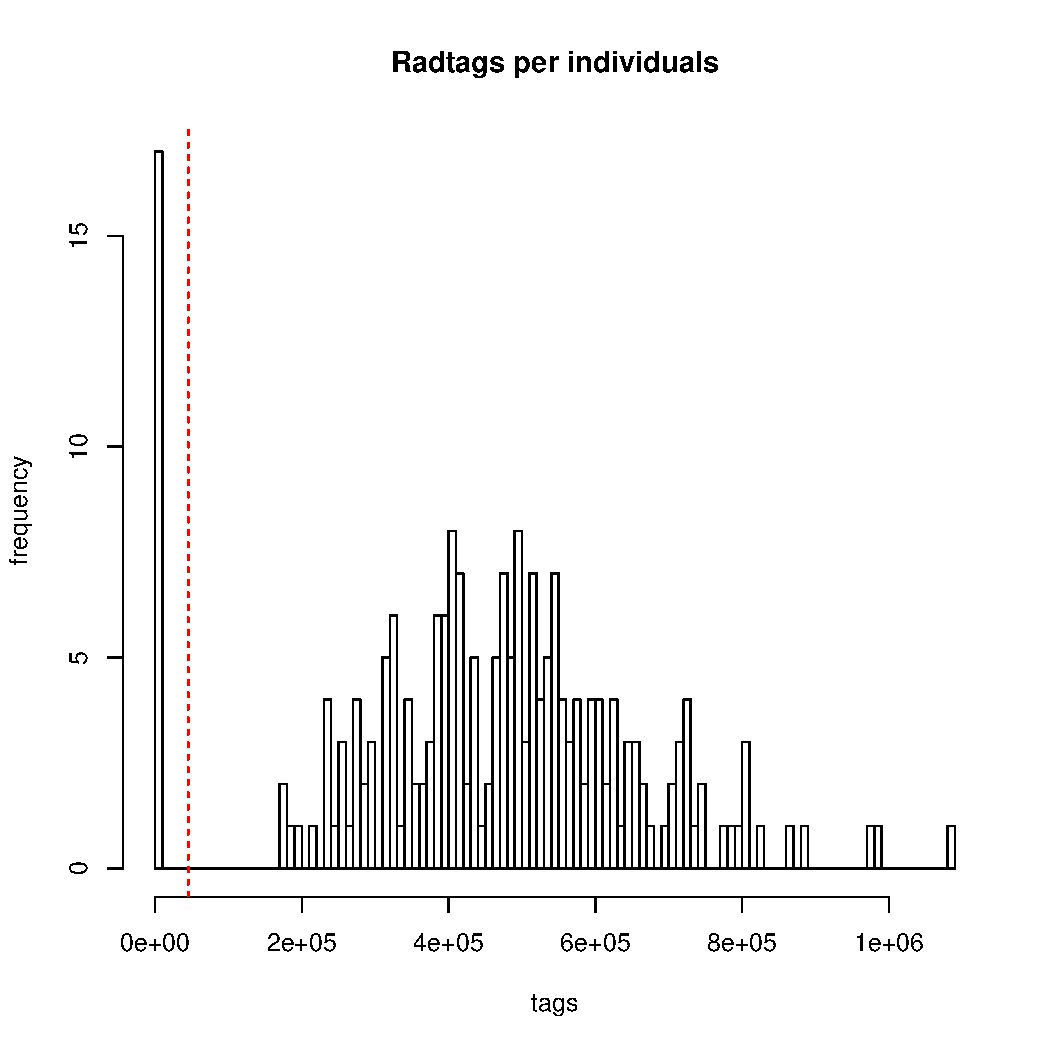
\includegraphics[width=0.7\textwidth]{stacks_pipeline/radtags_distrib.pdf}
		\caption{distribution of the number of radtags (reads) per sample. The red vertical dashed line indicates the cutoff value set to 10\% of the mean. Samples below this value are removed from the analysis.}
		\label{tags_dist}
	\end{center}
\end{figure}
\FloatBarrier
Summary results with n=1:
\begin{itemize}
\item All non-empty samples (198): 25618 alleles in catalogue, over 7062 loci.
\item Excluding samples with \textless 10\% of mean tags (185): 25585 alleles in catalogue, over 7046 loci
\end{itemize}

note: following recommandations from Paris et al. 2017, Lost in parameter space: a roadmap for STACKS. \textit{Methods in Ecology and Evolution}, I set the value of n to 3 (M-1=3)

\section{sstacks}

sstacks is used to generate one file per individual, in each file, the matching loci point to the cstacks catalogue. There is no crucial parameter to change in this program.

\section{populations}

The "populations" component of STACKS is used to compute population genetics statistics on a set of individuals. I use it here to compute FST statistics (fixation index) along the genome. It offers several features to compute different statistics, including a bootstrapping feature and a "kernel smoothing" flag, allowing to take neighbouring region into account with a decreasing weight as a function of their distance from the focus nucleotide. I will use both of these features to compute FST.

The main features to change in FST calculation are :
\begin{itemize}
\item -r: minimum percentage of individuals in a population required to process a locus for that population.
\item -p: minimum number of populations a locus must be present in to be procesed.
\item -m: minimum stack depth required for individuals at a locus.
\end{itemize}

Example populations call for FST calculation:
\begin{lstlisting}
$ populations -P <stacks_files> -M <popmap> -b 1
 -k -r 0.75 -f p_value
\end{lstlisting}

\subsection{populations results}

I ran populations with the following parameters:
\begin{itemize}
\item -r: 0.75 - 0.85
\item -p: 2
\item -m: 5
\end{itemize}

Therefore, only loci with at least 5 reads of coverage were included, each loci also needs to be in at least 75\% to 85\% of all individuals and in both populations (males and females).

This table summarizes the first statistics I extracted from the VCF files (using vcftools) with the different values for r:
\begin{center}
\vspace{10px}
\csvautobooktabular[respect underscore=true]{param_space/vcf_sumtable.csv}
\vspace{10px}
\end{center}

plotting the inbreeding coefficient per individual with r=75 yields:

\begin{figure}[h]
	\begin{center}
		\hspace*{-1in}
		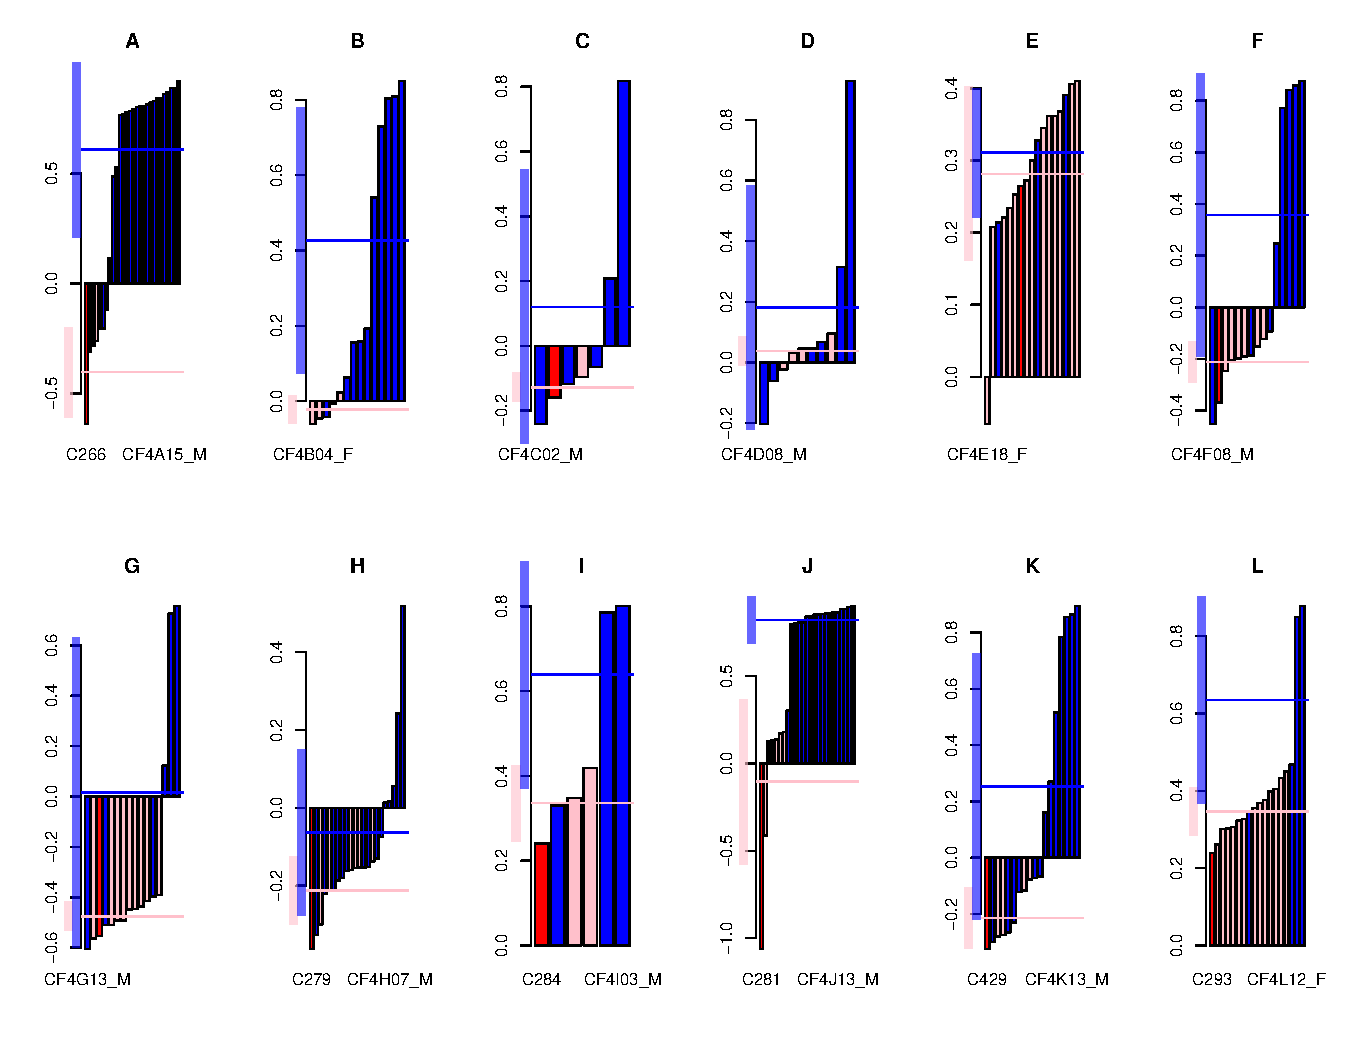
\includegraphics[width=1.5\textwidth]{F_d-25_r-75}
		\caption{Inbreeding coefficient (F). Each plot is a family, each bar is an individual. Blue bars represent males and pink ones represent females and red ones are mothers. color bars on the y axis span the mean +- standard deviation of males and females, respectively. In theory, mothers should have the lowest inbreeding coefficient of their family (highest heterozygosity)}
	\end{center}
\end{figure}

When increasing the minimum depth above ~15, populations crashed. Disabling bootsrapping and kernel smoothing fixed the issue. Guess: May be caused by a contig smaller than the sliding window size during kernel smoothing. This could be the case if the sliding window has a min number of loci, in which case increasing minimum depth would cause the window to enlarge.

I tested for correlations between Mean depth of loci and homozygosity in all individuals and per family, no significant correlation was found. This means there should not be significant allele excludion caused by too stringent min depth (i.e. stacks removed because of low coverage, resulting in homozygous loci).

\section{STACKS parameters summary}
\begin{table}[h!]
\begin{tabular}{c|c}
process radtags & Mis:2\\
bwa & Mis:4\\
Pstacks & MinDep:3\\
Cstacks & LocMis:1\\
Sstacks & -\\
populations & IndProp:0.75, MinDep:5(25)*, MaxHet:0.9\\
\vspace{5px}
\end{tabular}
\\
 \footnotesize * Stringent MinDepth value used to exclude haploid males. The smaller value is used for downstream analyses to keep more loci.
\end{table}

\FloatBarrier

\chapter{Excluding haploids}

I used the F statistics (coefficient of inbreeding) computed by vcftools to measure homozygosity levels in each individual. The F statistics used were generated with more stringent parameters (min depth: 25) to call ploidy more confidently. It is calculated as $F = \frac{O-E}{N-E}$ where O is the observed number of homozygous loci, E is the number expected by chance and N is the total number of loci.

First, I calculated the Mean $\mu$ and standard deviation $\sigma$ of the inbreeding coefficient $F$ among daughters in each family. I then classified males with:
\\
\begin{center}
 $F > \mu + 2\sigma $  \\
\end{center}

 as haploid. This is stringent threshold should exclude all haploid males, but it can also potentially exclude diploid males from the analysis.

Update: 08.06.2017

I tried 12 different thresholds for excluding haploids. The thresholds were computed according to these rules:
\begin{itemize}
\item 1: All thresholds follow the formula $\mu + \tau(N\sigma)$ with $1 \leq N \leq 4$
\item 2:  $1 \leq \mu \leq 4$
\item 3: $\tau$ is a function for transforming the inbreeding coefficient values. Either $\tau(F) = F^2$ or $\tau(F) = \sqrt{F}$
\end{itemize}
As shown above, in this report I will use the threshold named "m2" which corresponds to  $F > \mu + 2\sigma $.
Figure \ref{haplodiplo} shows a plot showing the separation of haploid and diploids using this threshold.

\begin{figure}[h]
	\begin{center}
		\hspace*{-0.8in}
		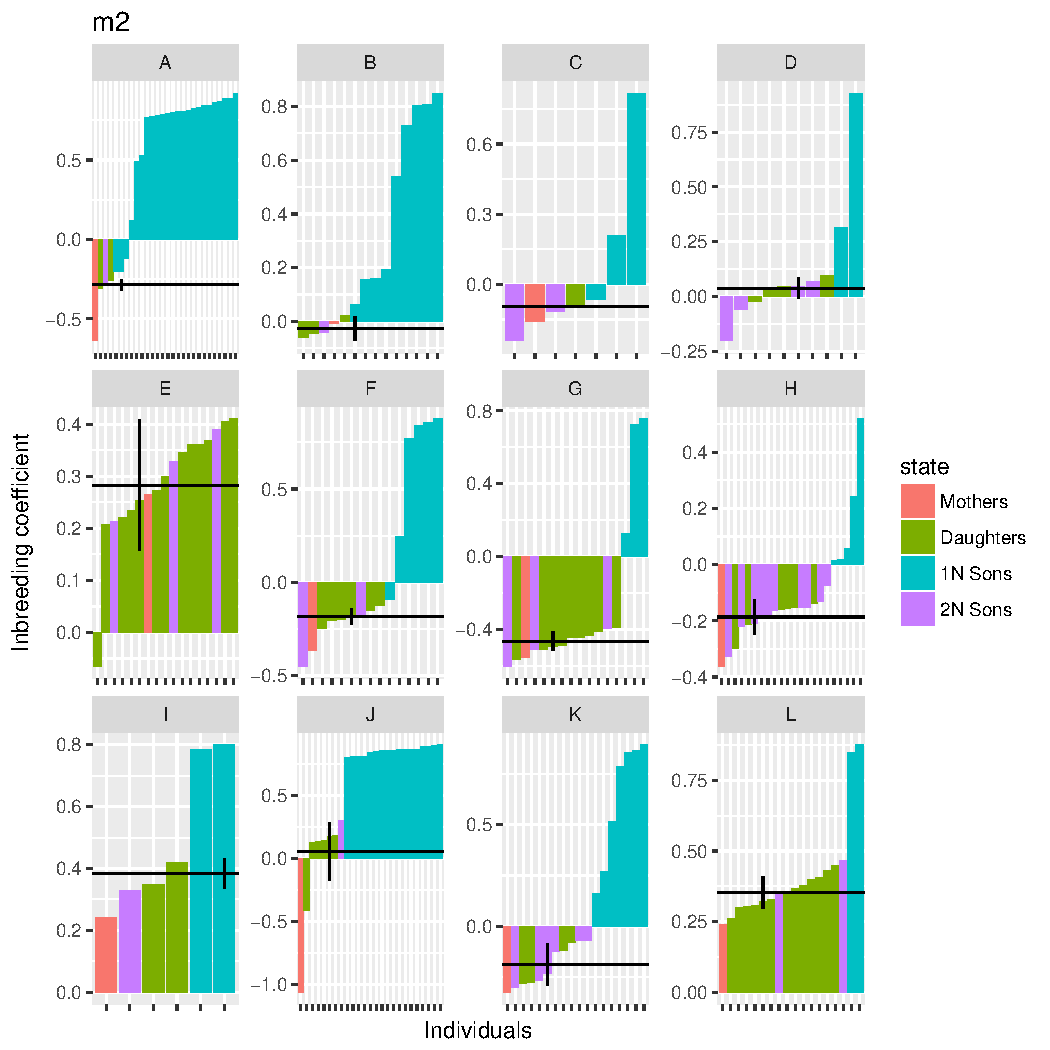
\includegraphics[width=1.2\textwidth]{exclu_haplo/m2}
		
		\caption{Inbreeding coefficient (F). Different colors represent the different types of individuals, as shown in the legend. Each plot is a family, each bar is an individual. Horizontal black bars show the mean inbreeding coefficient of daughters within the family $+/-$ the standard deviation (vertical black line). In theory, mothers should have the lowest inbreeding coefficient of their family (highest heterozygosity)}
		\label{haplodiplo}
	\end{center}
\end{figure}

\FloatBarrier

After separating haploids from diploids, I performed exploratory analyses prior to association mapping. The goal of these is to assess the homozygosity rate of SNPs in diploid males and females and how many seem to fit the CSD pattern. As shown in Figure \ref{SNPs_explo5} and \ref{SNPs_explo25}, there is no single SNPs thatis heterozygous in all females and homozygous in all diploid males. That can imply that the species has ml-CSD and there is no single locus that always fit the CSD pattern, or the restriction enzyme used in the RAD-seq protocol (ecoR1) did not cut in the CSD locus directly. It is very likely a combination of both explanations. It is also worth mentioning that, besides the number of SNPs, it makes little difference whether I use permissive (Figure \ref{SNPs_explo5}) or stringent (Figure \ref{SNPs_explo25}) parameters. The only notable change is that including more SNPs results in higher homozygosity for both sexes.

In this analysis, I excluded all consensus loci (where all individuals had the same allele) and did not consider SNPs with more than 2 genotypes in a single individuals in the heterozygosity calculation (counted as missing values), as they are likely due to contaminations.

\begin{figure}[h]
	\begin{center}
		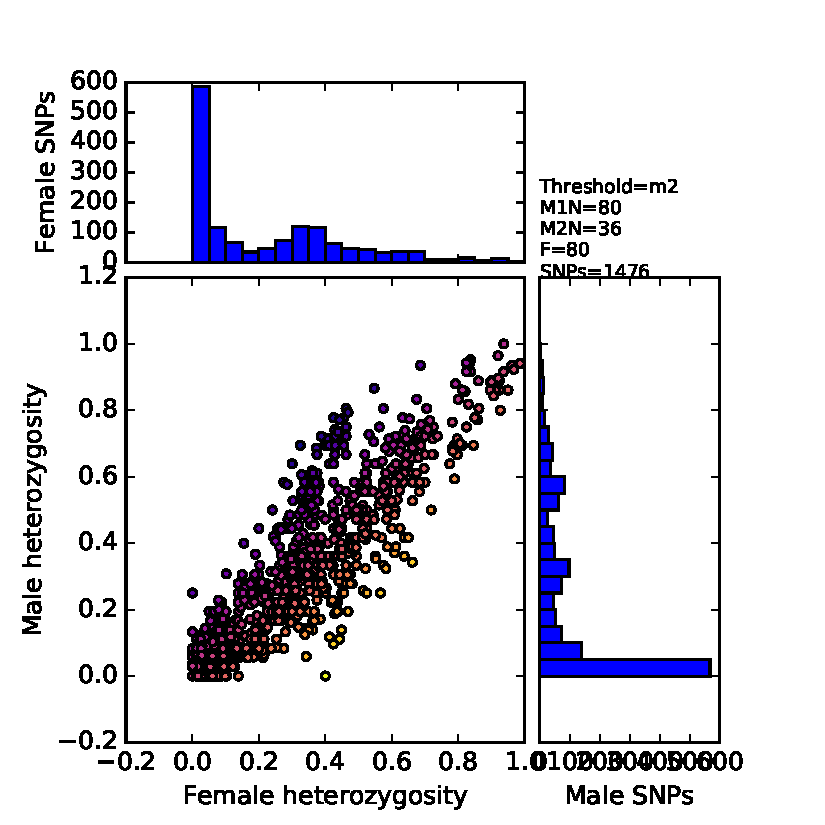
\includegraphics[width=0.8\textwidth]{exclu_haplo/d5assoc_explo/m2}
		\caption{Homozygosity of female and diploid male SNPs where depth $\geq 5$ (permissive parameters). Each point on the scatterplot is a SNP, and its coordinate are the proportion of females (x) and males (y) in which it is homozygous. Histograms allow to visualize the distribution of homozygosity for SNPs of each sex. The color code shows how SNPs fit the CSD pattern with lighter points being closer to it (i.e. more homozygous in males and heterozygous in females). Summary statistics on the top right show the threshold used, the number of haploid males excluded (M1N) as well as the number of diploid males (M2N), females (F) and SNPs included.}
		\label{SNPs_explo5}
	\end{center}
\end{figure}

\begin{figure}[h]
	\begin{center}
		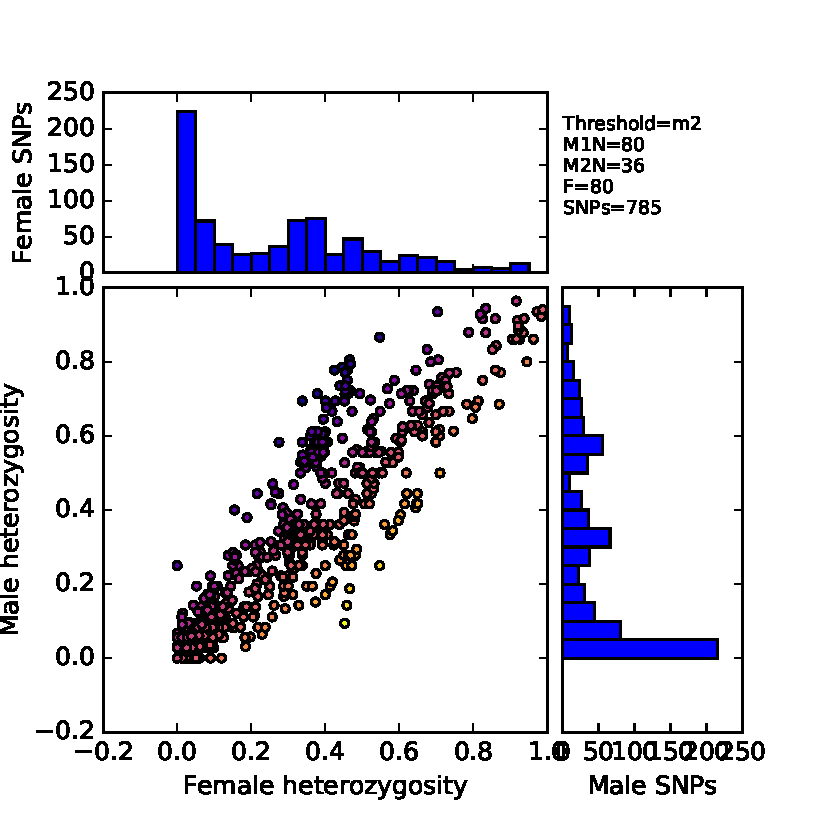
\includegraphics[width=0.8\textwidth]{exclu_haplo/d25assoc_explo/m2}
		\caption{Homozygosity of female and diploid male SNPs $\geq 25$ (stringent parameters). Each point on the scatterplot is a SNP, and its coordinate are the proportion of females (x) and males (y) in which it is homozygous. Histograms allow to visualize the distribution of homozygosity for SNPs of each sex. The color code shows how SNPs fit the CSD pattern with lighter points being closer to it (i.e. more homozygous in males and heterozygous in females). Summary statistics on the top right show the threshold used, the number of haploid males excluded (M1N) as well as the number of diploid males (M2N), females (F) and SNPs included.}
		\label{SNPs_explo25}
	\end{center}
\end{figure}


\FloatBarrier

\chapter{Cleaning genomic data}

date : 23.06.2017
\\

The first attempt at separating individuals based on inbreeding coefficient revealed several issues inherent to the data:
\begin{itemize}
\item The inbreeding coefficient is not clearly bimodal in all families (1 haploid mode and 1 diploid mode)
\item Some loci have more than 2 haplotypes, although we are working with diploids.
\item There are no loci that clearly stand out as perfectly 'CSD like' among all individuals, this should be looked at family-wise.
\end{itemize}
These issues will be solved one by one in this chapter.

\section{Improving ploidy separation metric}

The inbreeding coefficient was computed using all males/females. Also, the raw heterozygosity may be a more accurate metric than inbreeding coefficient. Both issue require the analysis to be done in a per-family fashion, either by re-running the populations program for each family, or implementing family as an additional population layer.
\\
Date: 27.06.2017
\\
Solution: I could switch to observed homozygosity, but I think it is also fine to keep this metric (I can always change it later). I did however, re-run the populations program separately for each family. I did not add a population layer to the popmap, because it would not have allowed for different loci blacklists between families when solving the third issue. Visualizing the distribution of inbreeding coefficients across individuals reveals a pretty good (?) separation of individuals (Figure \ref{ploidy_metric}).


\begin{figure}[h]
	\begin{center}
		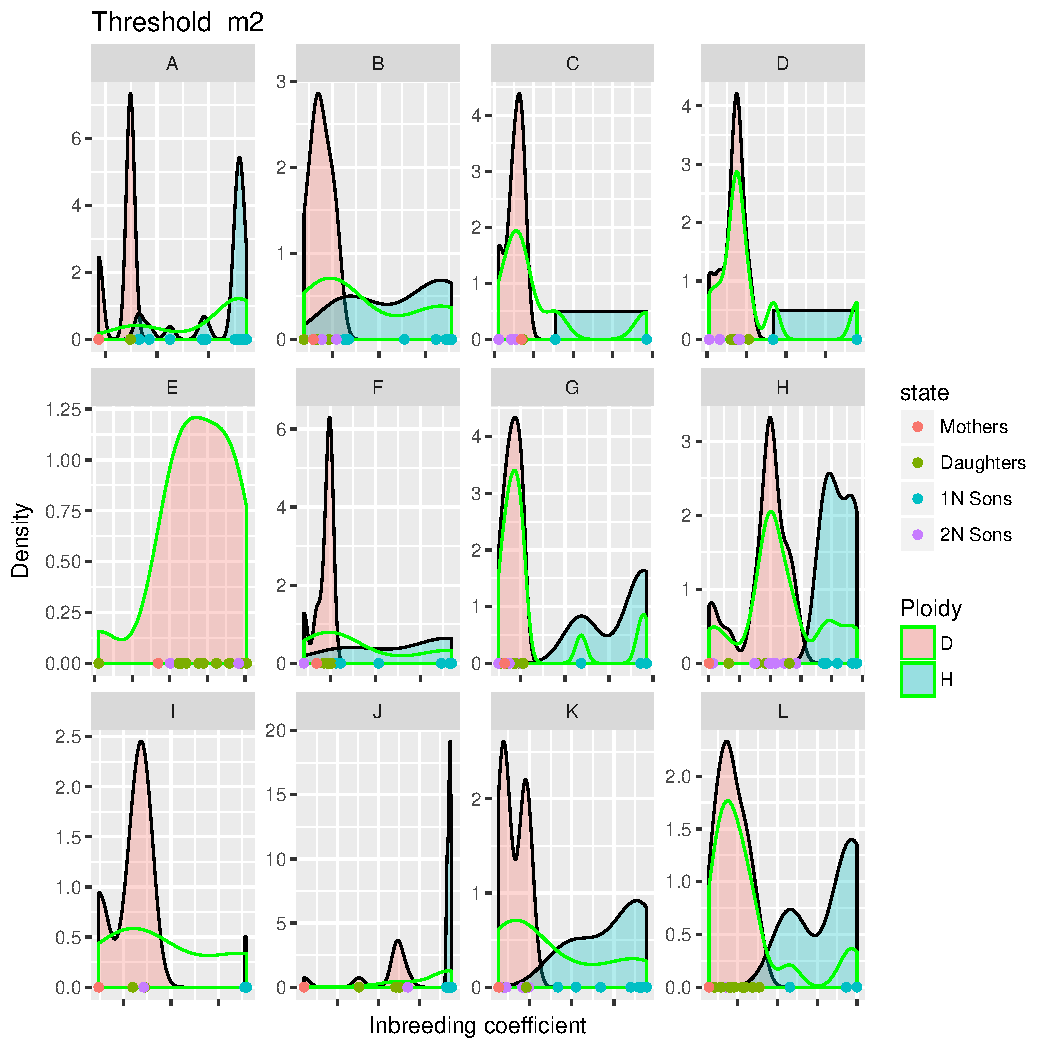
\includegraphics[width=0.8\textwidth]{cleaning_genomic_data/F_r-75_d-5_m2_density.pdf}
		\caption{Distriution of individual inbreeding coefficient. The green curve represents the overall distribution of inbreeding coefficients within the family. The blue and pink areas represent the distribution of inbreeding coefficients for haploids and diploids, respectively, split using the m2 threshold defined at the beginning of chapter 4. Ideally, the green curve would follow a bimodal distribution clearly separating individuals by homozygosity.}
		\label{ploidy_metric}
	\end{center}
\end{figure}

Date: 12.07.2017
Update: This method of ploidy separation is flawed as it will overestimate the number of haploid males in families with few females. Indeed, with a lower standard deviation of female homozygosity, the threshold tends to the mean only.

Because the homozygosity of diploid offspring depends on its mother, but that of haploids are independent of mother background, I can probably use a universal threshold for all families. This way, the threshold can be equally conservative in all families and not biased towards certain of them. Plotting homozygosity of all individuals (Figure \ref{ploidy_fixed}) revealed 2 separate meta-distributtions. The one on the left is a gaussian made up of several smaller ones (each smaller distribution is a family, with the mean depending on the mother), whereas the distribution on the right is made of a single gaussian containing all (or most) haploid males.
Choosing a fixed conservative threshold in between should allow to keep more individuals and remove bias.

\begin{figure}[h]
	\begin{center}
		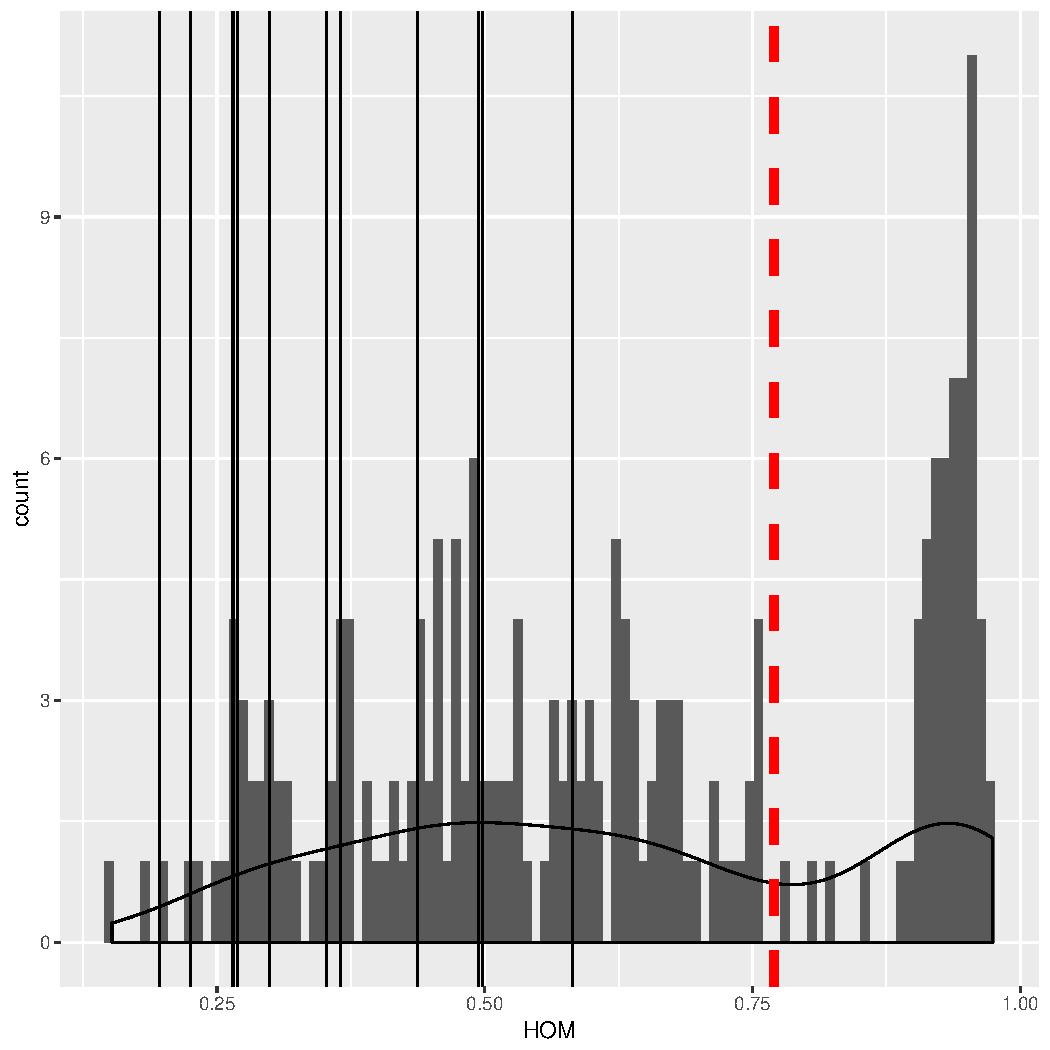
\includegraphics[width=0.8\textwidth]{cleaning_genomic_data/ploidy_sep_fixed.pdf}
		\caption{Distribution of the proportion of homozygous loci across all individuals. Continuous vertical black lines are the mothers values and the dashed vertical red line is the (visually) optimal threshold, fixed at 0.77.}
		\label{ploidy_fixed}
	\end{center}
\end{figure}

\section{Loci with 3 or more haplotypes}

There are two possible explanation for the existence of these loci. It could be either due to a contamination, in which case few individuals would present many loci with 3 or more haplotype. On the other hand, if few loci have this issue in several individuals, it could be due to paralog merging. This can be solved by identifying which case is the most likely, and either excluding concerned individuals (first case), or loci (second case).

24.06.2017: Asked on STACKS google group about the haplotypes.tsv file. It is apparently normal to have more than 2 genotypes and depends on the parameters that were set in pstacks/ustacks. The answer I got, is that I should only work with the VCF file, which calls only 2 genotypes/site/individual. This imply figures \ref{SNPs_explo25} and \ref{SNPs_explo5} are not valid, as I misinterpreted the file content. I will re-generate these figures using the VCF file directly.
\\
Date: 27.06.2017
\\
Solution: I used the -012 argument in VCFtools to produce a genotype matrix from the populations output VCF file. This matrix encodes the genotype of each individual at each SNP with an integer representing the number of non-reference alleles present. These matrices were generated separately for each family and used to regenerate the figures \ref{SNPs_explo25} and \ref{SNPs_explo5}.

The issue when visualizing the SNPs heterozygosity per family (Figure \ref{SNPs_explo_fam}) is that the low number of individuals allow for few different heterozygosity values for any given SNPs, yielding a high number of 'perfectly' CSD-like candidates. Solving the next issue or grouping SNPs by contig/locus may help reduce this number, but ultimately only association mapping will allow to find the best candidate region. 


\begin{figure}[h]
	\begin{center}
		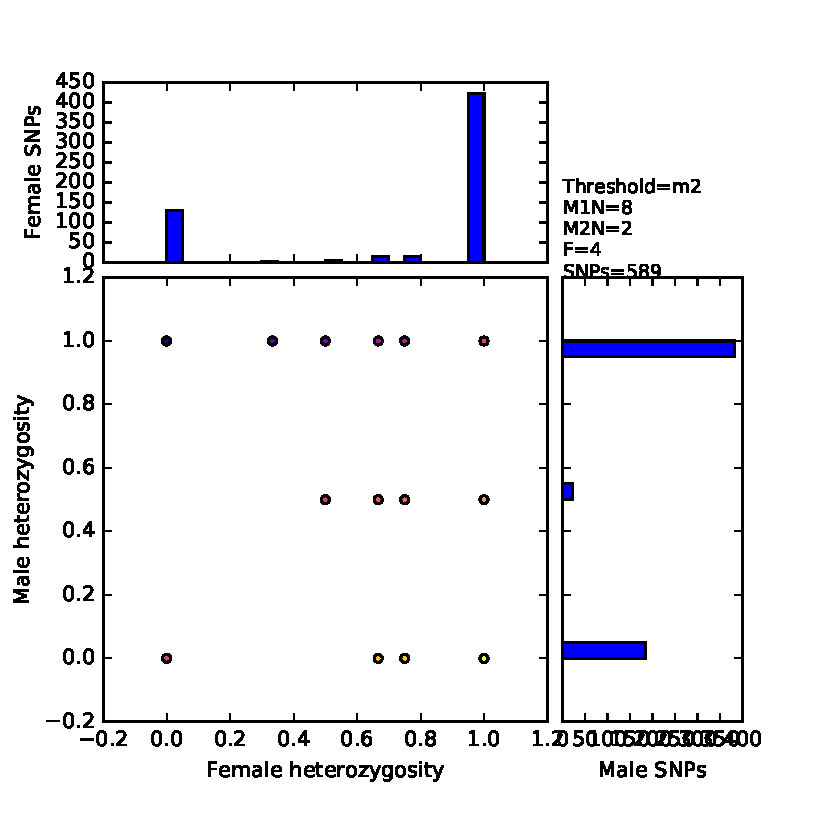
\includegraphics[width=0.8\textwidth]{cleaning_genomic_data/assoc_explo_fam/B.pdf}
		\caption{Example: SNPs heterozygosity across individuals of family B. The yellowness represents the proximity to CSD-like pattern (i.e. homozygous in all males and heterozygous in all females. Note: populations parameters set to : min depth (D)=5 and prop pop (r)=75}
		\label{SNPs_explo_fam}
	\end{center}
\end{figure}


\section{No clear signal in whole population}

This issue could be expected from the biological system because it is believed that there is ml-CSD in this species; there should be no single locus that will fit the CSD pattern across all individuals. This mean we need to identify different loci independently in each family. There are several things which can be done to work around this issue. 

First, and most importantly, the populations program should be taking family information into account, but this was done already when solving the first issue (Improving ploidy separation metric). Second, the data should be cleaned by blacklisting loci that are homozygous in mothers in each family, as there is no way these will be heterozygous in their respective daughters and be CSD candidates.
\\
Date: 29.06.2017
\\
Solution: I re-ran the explo assoc script used to generate figure \ref{SNPs_explo_fam} and excluded all SNPs that are homozygous in the mother (Figure \ref{SNPs_explo_nomother}). It removed a significant number of SNPs from the set, but there are still way too many that fit the CSD pattern.

\begin{table}
	\begin{center}
		\csvautobooktabular[respect underscore=true]{cleaning_genomic_data/hom_mother.txt}
		\caption{Number of homozygous SNPs found in the mother of each family. Note family D is excluded since there was no genomic data available for this mother.}
		\label{hom_mother}
	\end{center}
\end{table}

\begin{table}
	\begin{center}
		\csvautobooktabular[respect underscore=true]{cleaning_genomic_data/CSD_like.txt}
		\caption{Number of homozygous SNPs that fit the CSD pattern in each family.}
		\label{CSD_like_raw}
	\end{center}
\end{table}


\begin{figure}[h]
	\begin{center}
		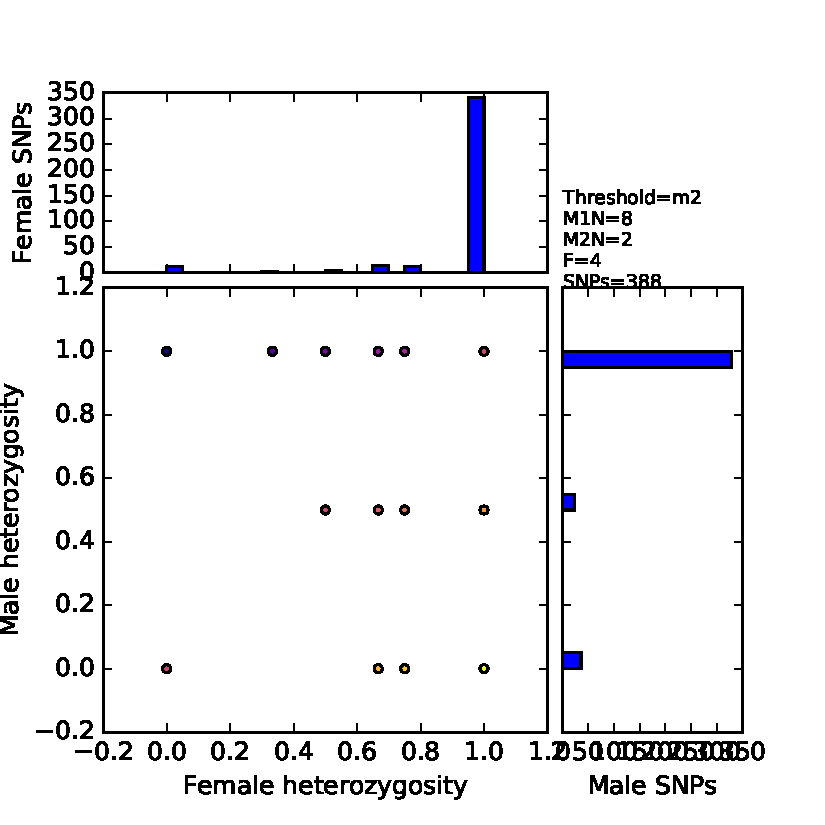
\includegraphics[width=0.8\textwidth]{cleaning_genomic_data/assoc_explo_fam_no_mother/B.pdf}
		\caption{Example: SNPs heterozygosity across individuals of family B after removing SNPs that are homozygous in the mother. The yellowness represents the proximity to CSD-like pattern (i.e. homozygous in all males and heterozygous in all females. Note: populations parameters set to : min depth (D)=5 and prop pop (r)=75}
		\label{SNPs_explo_nomother}
	\end{center}
\end{figure}
\FloatBarrier


Date: 24.07.2017

I removed loci that are homozygous in mother using a second technique: 
\begin{itemize}
\item For each mother: use Pstacks snps file to find sample ID of all loci for which all position are "O" (for homozygous).
\item Look up the sstacks matches file of each mother to retrieve the matching catalog ID
\item exclude corresponding catalog ID for the family in populations output files in downstream analyses.
\end{itemize}

I am still not sure if this technique is safe / correct, the steps described above are currently implemented in the hom_filt function of Hom\_M-F.R.

Date: 28.07.2017

I am noww using a much simpler method which should be  relatively correct. I use the output populations file "batch_0.sumstats.tsv" to remove the SNPs that have no alternative nucleotide in the female population. I am therefore
assuming that if the mother is homozygous, all daughters are as well. That means I might keep some SNPs that are in fact homozygous in the mother, either due to sequencing errors or point mutations, but these events should be extremely rare.

\subsection{Transmission bias}

Here I check how frequently SNPs that are homozygous in a mother are heterozygous in its offspring and vice versa.
(to be continued)

\chapter{Association mapping}

Date: 05.07.2017

Now that the data is cleaner, I will start with the association mapping. Casper provided me the genome with the contigs ordered by chromosomes (but not oriented?) he obtained with his linkage map. I will use this as the new reference genome and run the pipeline all the way from the mapping with it.

Date : 08.07.2017

I ran the whole pipeline on the ordered genome. Here are all statistics associated with all steps of the analysis previously described.\\
\FloatBarrier

\begin{table}[h]
\csvautobooktabular[respect underscore=true]{association_mapping/ref_genome_stats.csv}
\caption{Assembly statistics for the ordered reference genome of \textit{Lysiphlebus fabarum}}
\label{assembly_stats_ordered}
\end{table}

\begin{table}[h]
\csvautobooktabular[respect underscore=true]{association_mapping/mapstats.csv}
\caption{Mapping: Proportion and number of reads aligned on the ordered reference genome using BWA's aln algorithm with 4 mismatches allowed.}
\label{mapping_stats}
\end{table}

\begin{table}
\csvautobooktabular[respect underscore=true]{association_mapping/pstats.csv}
\caption{Pstacks: Summary statistics of stacks obtained with minimum coverage set to 3 in pstacks, using the ordered genome.}
\label{pstacks_ordered}
\end{table}

\begin{table}
\csvautobooktabular[respect underscore=true]{association_mapping/cstats.csv}
\caption{Cstacks: Summary statistics of loci obtained with a mismatch value set to 3 in cstacks using the ordered genome.}
\label{cstacks_ordered}
\end{table}

\FloatBarrier

\section{Coarse analyses}
Before running any association mapping analysis, I will blacklist loci that are homozygous in mothers and individuals that are defined as haploids with m2 homozygosity threshold from the populations analysis and rerun it.

\section{Number of CSD loci}

It is possible to approximate the number of CSD loci heterozygous in a mother using the proportion of males among diploid individuals. Provided the loci are on different chromosomes, if n CSD loci are heterozygous in the mother, there should be $\frac{1}{2^n}$ of males among diploid, because as long as heterozygosity is retained at one of these loci, the offspring should be female.

I changed the method of ploidy separation to a fixed threshold of homozygosity identical for all families, since homozygosity of haploid males should not depend on their mother's genetic background. This should provide an unbiased (or equally biased) proportion of males in all families.

Once the mothers have been categorized based on the proportion of males in their diploid offspring, I will use this category information to filter loci that are homozygous in mothers with more loci ? not sure...

\chapter{Male-Female Fst}

Date: 17.07.2017\\
During preliminary analyses, I noticed recurrent peaks in Fst between diploid males and females in different families. This could indicate the presence of male-deleterious alleles. To further investigate this possibility, I analysed Fst again using all individuals (including haploids).

I first looked at Fst over all 6 chromosomes in the assembly, averaging the Fst at each SNP across family to have an overview (Figure \ref{haplo_Fst_avg}), and then splitting the families to identify recurrent peaks (Figure \ref{haplo_Fst_per_fam}).

\begin{figure}[h]
	\begin{center}
		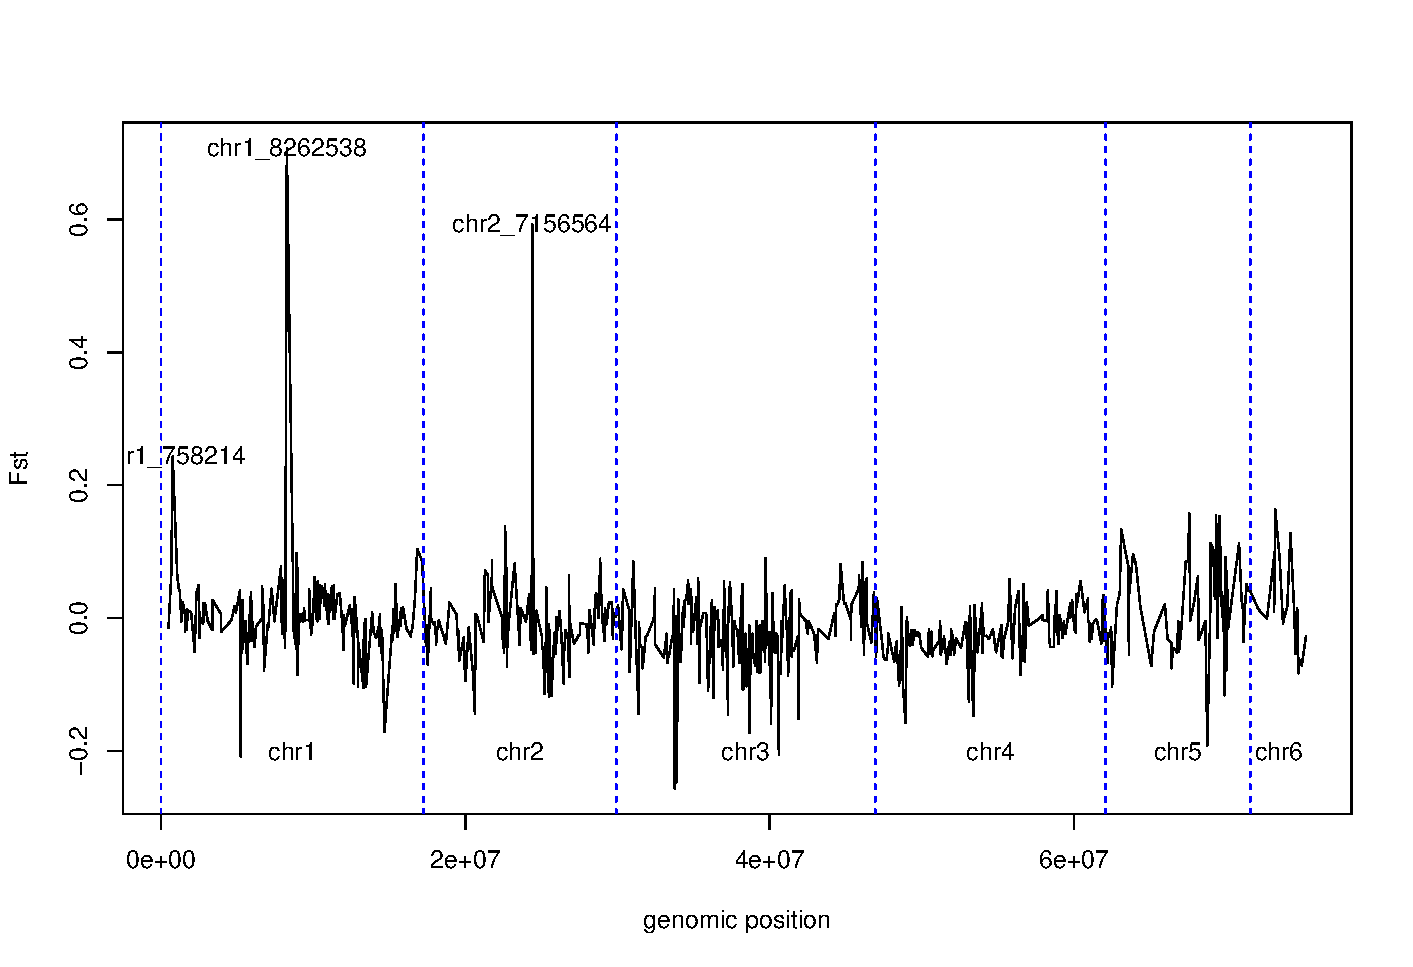
\includegraphics[width=0.8\textwidth]{association_mapping/haplo_avg_all_Fst.pdf}
		\caption{Fst values averaged at each SNP across all families. All individuals, including haploids and mothers are included in the analysis and top scoring peaks are labelled with the SNP position in the format "chromosome\_basepair" where basepair is the position within the chromosome. Note: populations parameters set to : min depth (D)=20 and prop pop (r)=80}
		\label{haplo_Fst_avg}
	\end{center}
\end{figure}

\begin{figure}[h]
	\begin{center}
		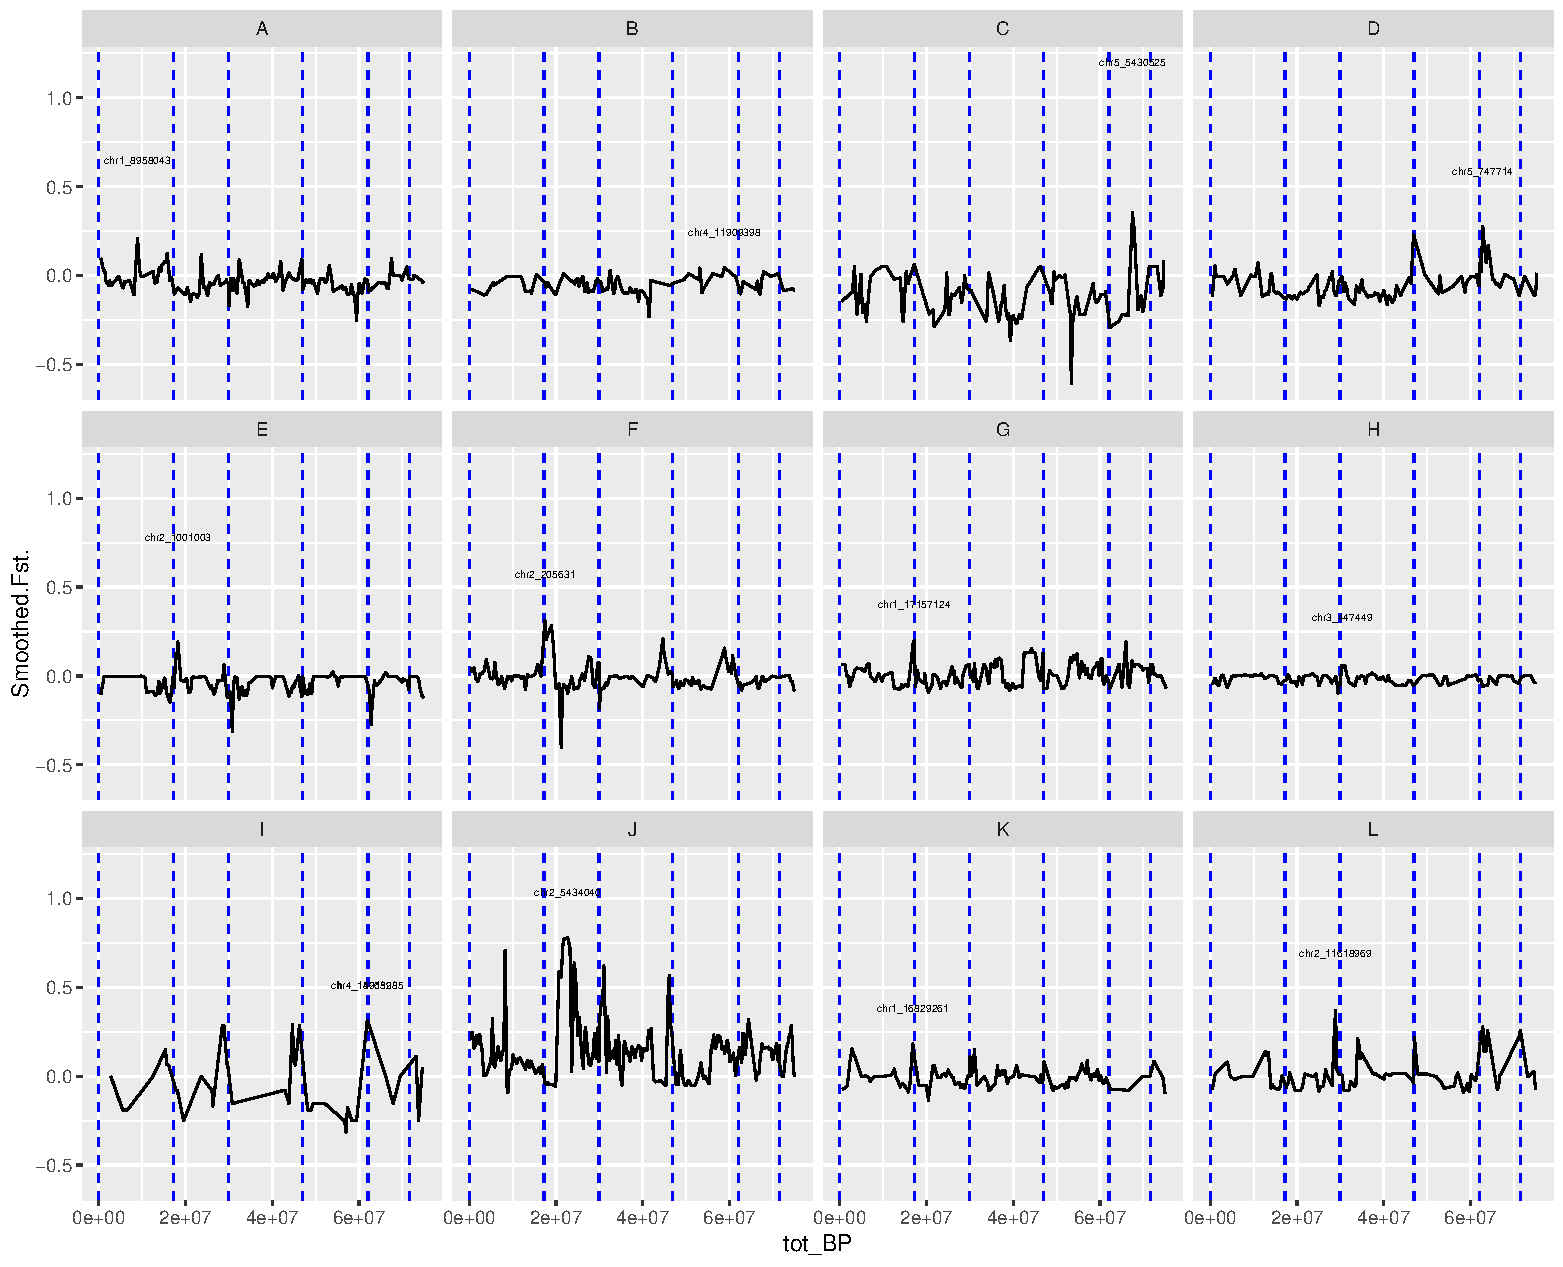
\includegraphics[width=\textwidth]{association_mapping/haplo_Fst_per_fam.pdf}
		\caption{Fst values at each SNP by family. All individuals, including haploids and mothers are included in the analysis and top scoring peaks are labelled with the SNP position in the format "chromosome\_basepair" where basepair is the position within the chromosome. Note: populations parameters set to : min depth (D)=20 and prop pop (r)=80}
		\label{haplo_Fst_per_fam}
	\end{center}
\end{figure}
\FloatBarrier

The issue with averaging the Fst over families as in figure \ref{haplo_Fst_avg} is that some SNPs can be sequenced in only one family, therefore the averaged value will only depend on that family. If we merge all families' curve into a single plot, it appears there is no single peak common to all families. 
This can either mean that there is no interesting signal, or if that the signal depends on the family's genetic background, possibly due to an epistatic effect. Here, however, I do not have the sample size to test for it. 

\section{TO DO}
\begin{itemize}

\item FOR MONDAY : nice table with all offspring numbers (1NM, 2NM, F) per family to determine with Casper where and how many individuals we need to add in existing families.
\item identify metacentric and telocentric chromosomes using proportion of homozygous offspring at each SNP along genome. (proportion should either increase or decrease towards ends of chromosomes.
\item use proper visualization technique with a smoothed trend line weighted by the number of offspring supporting each SNPs.
\item classify families by proportion of males among diploid offspring. The proportion of males should indivate different combination of CSD loci. Recombination rates will vary depending on distance from centromere
\item Find CSD peaks that are intersect in several families ?
\item if n CSD loci on different chromosomes are het. in a mother, the proportion of males in diploid offspring will be $\frac{1}{2^n}$. 
\item Compute coverage along genome for all loci including monomorphic ones.
\item Isolate regions of abnodmally high coverage, eventually exclude them. Watch out for overmerging of paralogs and repetitive sequences.
\item Visualize average heterozygosity (or allele frequency) at each SNPs in offpring versus in mother to assess transmission bias (hom SNPs in mothers more often het in offspring or reversse). 
\item Validate haploid definition using haplotypes deduced from linkage map.
\item convert VCF file into PED format using vcftools
\item import data into genABEL and perform association mapping
\end{itemize}

\end{document} 
\grid
%                                 